% Slide: Tổng quan
\begin{frame}{Python server: Tích hợp và Phát hiện}
    \begin{block}{Tổng quan}
        \begin{itemize}
            \item Hệ thống Python tích hợp dữ liệu từ:
            \begin{enumerate}
                \item \textbf{ESP32}: Trạng thái té ngã, GPS qua MQTT.
                \item \textbf{Camera IP}: Phát hiện người, theo dõi, ước lượng tư thế bằng AI.
            \end{enumerate}
            \item Đồng bộ, tích hợp dữ liệu để phát hiện té ngã, gửi cảnh báo, lưu sự kiện.
        \end{itemize}
    \end{block}
    \label{sec:server_overview}
\end{frame}

% Slide: Kiến trúc hệ thống
\begin{frame}{Python server: Kiến trúc}
    \begin{block}{Mô hình phân tầng}
        \begin{itemize}
            \item \textbf{Lớp thu nhận}: 
                \begin{itemize}
                    \item \texttt{comm/}: MQTT, Telegram Bot, AMI.
                    \item \texttt{detection/}: Xử lý video, phát hiện người, theo dõi.
                \end{itemize}
            \item \textbf{Lớp xử lý}: \texttt{fall/}, \texttt{processing/} tích hợp qua \texttt{DetectionProcessor}.
            \item \textbf{Lớp đầu ra}: \texttt{database/} lưu \texttt{fall\_events.db}, \texttt{comm/} gửi cảnh báo.
        \end{itemize}
    \end{block}
    \label{subsubsec:system_overview}
\end{frame}

% Slide: Cấu trúc thư mục dự án
\begin{frame}[fragile]{Python server: Cấu trúc Thư mục}
    \renewcommand{\baselinestretch}{0.8}
    \begin{minted}[fontsize=\scriptsize, breaklines, bgcolor=lightgray]{text}
intergrate_fall/
├── comm/ (MQTT, Telegram, AMI)
├── config/ (cấu hình)
├── database/ (fall_events.db)
├── detection/ (human, tracker)
├── fall/ (fall_detector.py)
├── processing/ (detection_processor.py)
├── utils/ (draw_utils.py)
├── models/ (yolov8n.pt)
├── tests/ (test_fall.py)
├── main.py
    \end{minted}
    \renewcommand{\baselinestretch}{1.0}
    \label{subsubsec:project_structure}
\end{frame}

% Slide: Luồng xử lý
\begin{frame}[fragile]{Python server: Luồng Xử lý}
    \begin{block}{Quy trình}
        \begin{enumerate}
            \item Thu nhận: ESP32 (MQTT), Camera IP (AI).
            \item Tích hợp: \texttt{DetectionProcessor} đồng bộ dữ liệu.
            \item Đầu ra: Lưu sự kiện, gửi cảnh báo qua AMI/Telegram.
        \end{enumerate}
    \end{block}
    \begin{figure}
        \centering
        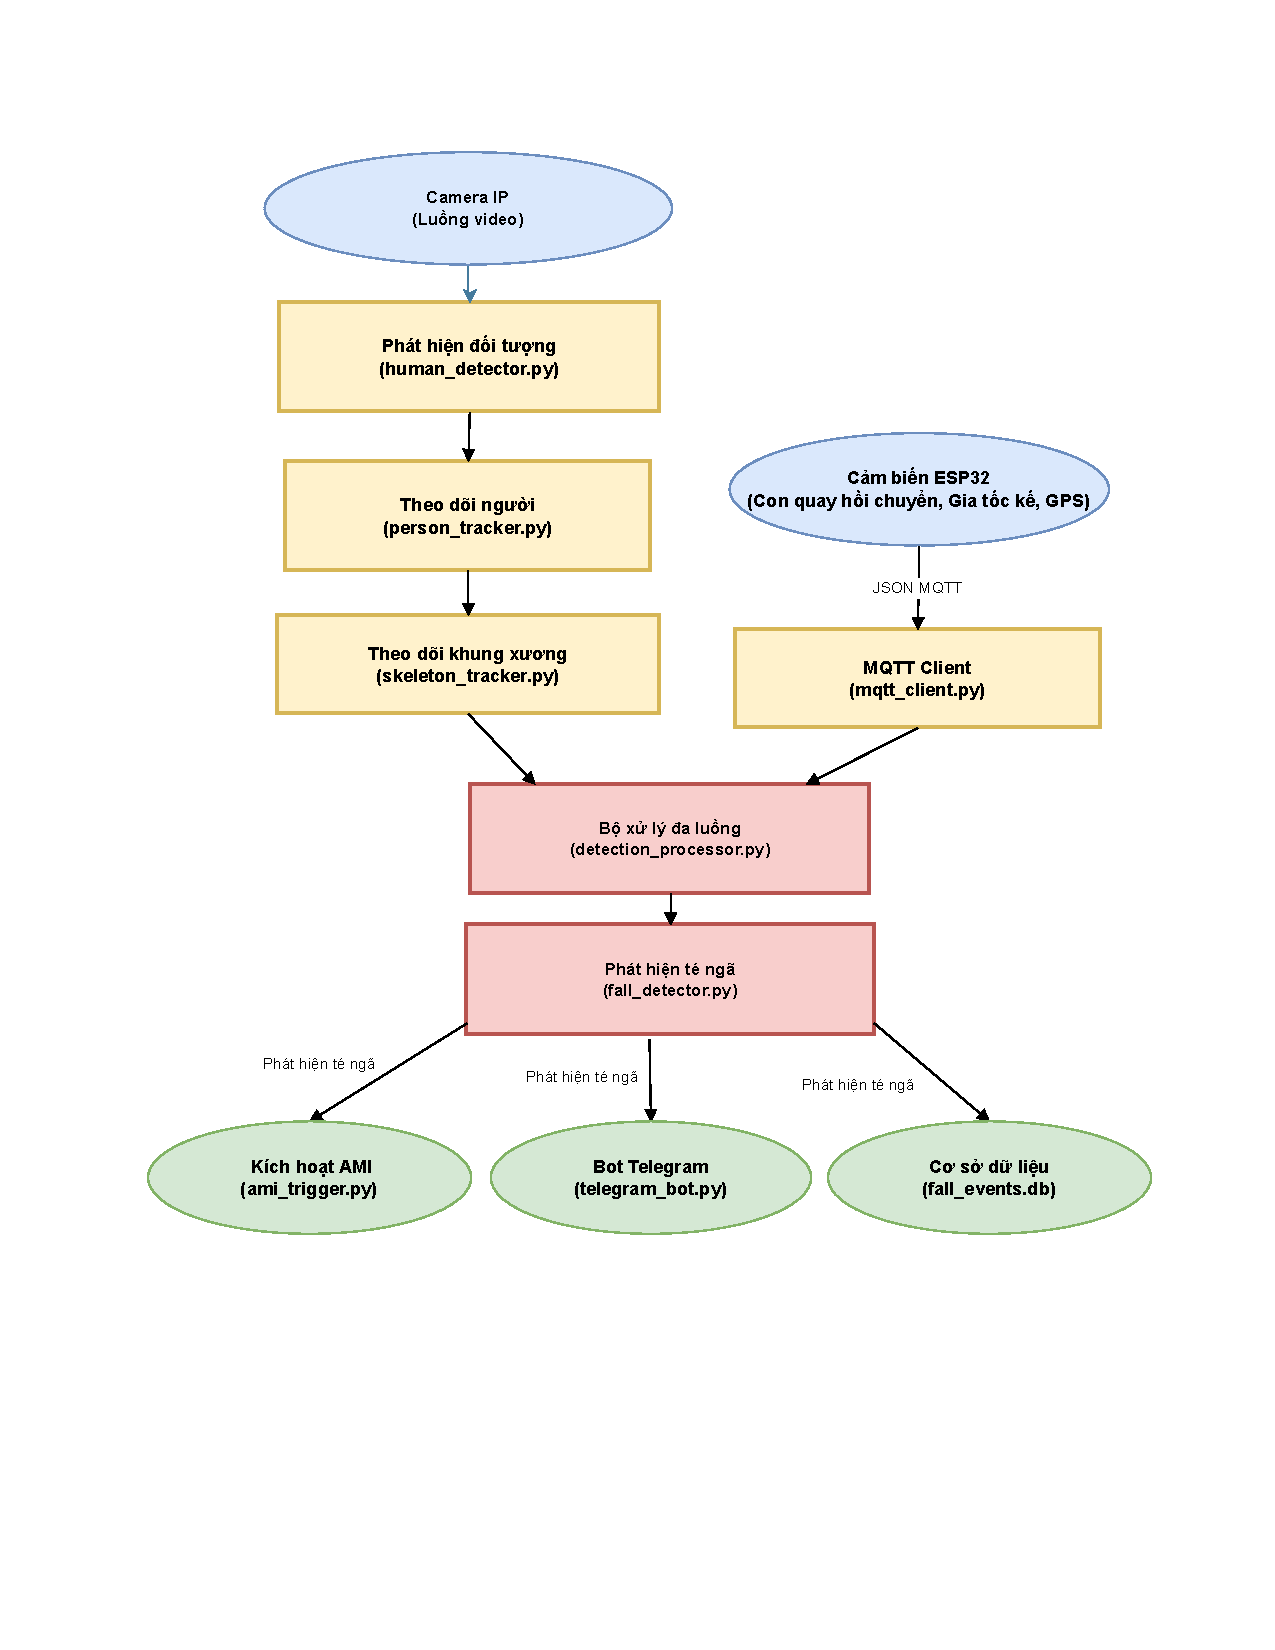
\includegraphics[width=0.85\textwidth,height=0.5\textheight,keepaspectratio]{images/server_flow.pdf}
        \caption{Luồng dữ liệu qua \texttt{DetectionProcessor}.}
        \label{fig:server_flow}
    \end{figure}
\end{frame}

% Slide: Kết hợp dữ liệu đa phương thức
\begin{frame}[fragile]{Python server: Tích hợp Dữ liệu}
    \begin{block}{Quy trình}
        \begin{itemize}
            \item Xác thực: ESP32 (\texttt{device\_id}, \texttt{fall\_detected}, GPS).
            \item Xử lý camera: Phát hiện người, ước lượng tư thế.
            \item Đồng bộ: Kiểm tra timestamp, cooldown (5 phút).
            \item Cảnh báo: AMI, Telegram (thử lại nếu lỗi).
        \end{itemize}
    \end{block}
    \begin{minted}[fontsize=\scriptsize, breaklines, bgcolor=lightgray]{python}
async def handle_camera_data(self, frame, person_id, box, landmarks):
    entity_id = f"camera_person_{person_id}"
    detector = self._get_or_create_detector(entity_id)
    is_fall = detector.detect_fall(landmarks)
    if is_fall and self._can_alert(entity_id):
        fall_event = self._create_fall_event("camera", entity_id, 0, 0, False)
        fall_id = await self._insert_fall_event_with_retry(fall_event)
        alert_msg = f"Fall detected by camera for {entity_id}. ID: {fall_id}"
        await self._send_alerts(alert_msg, frame)
    \end{minted}
    \label{subsubsec:multi_input_fusion}
\end{frame}

% Slide: Thuật toán phát hiện té ngã
\begin{frame}{Python server: Thuật toán Phát hiện}
    \begin{block}{Quy trình trong \texttt{FallDetector}}
        \begin{itemize}
            \item \textbf{Kiểm tra}: Landmarks hợp lệ (độ tin cậy $\geq 0.5$).
            \item \textbf{Tính toán}: 
                \begin{itemize}
                    \item Góc thân người: Dọc ($>60^\circ$), ngang ($>45^\circ$).
                    \item Vận tốc: Dịch chuyển thân người ($>0.5$ đơn vị).
                \end{itemize}
            \item \textbf{Trạng thái}:
                \begin{itemize}
                    \item \textit{Falling}: Góc và vận tốc vượt ngưỡng.
                    \item \textit{Lying}: Góc vượt ngưỡng kéo dài.
                \end{itemize}
            \item \textbf{Quyết định}: Bộ đếm $\geq 5$ frame → té ngã, đặt lại trạng thái.
        \end{itemize}
    \end{block}
    \label{subsubsec:fall_detection_algorithm}
\end{frame}

% Slide: Lưu đồ thuật toán
\begin{frame}[fragile]{Python server: Lưu đồ Thuật toán}
    \begin{figure}
        \centering
        \includegraphics[width=0.85\textwidth,height=0.7\textheight,keepaspectratio]{images/python_fall_diagram.pdf}
        \caption{Luồng thuật toán phát hiện té ngã.}
        \label{fig:python_fall_diagram}
    \end{figure}
\end{frame}

% Slide: Lưu trữ và cảnh báo
\begin{frame}[fragile]{Python server: Lưu trữ và Cảnh báo}
    \begin{block}{Cơ chế}
        \begin{itemize}
            \item \textbf{Lưu trữ}: SQLite \texttt{fall\_events.db} (timestamp, source, entity\_id, GPS).
            \item \textbf{Cảnh báo}: AMI, Telegram khi phát hiện té ngã.
            \item \textbf{Vòng lặp}: Thu thập → Xử lý → Tích hợp → Cảnh báo.
        \end{itemize}
    \end{block}
    \begin{minted}[fontsize=\scriptsize, breaklines, bgcolor=lightgray]{sql}
CREATE TABLE fall_events (
    id INTEGER PRIMARY KEY AUTOINCREMENT,
    timestamp DATETIME DEFAULT CURRENT_TIMESTAMP,
    source TEXT NOT NULL,
    entity_id TEXT NOT NULL,
    fall_detected BOOLEAN NOT NULL,
    latitude REAL,
    longitude REAL,
    has_gps_fix BOOLEAN,
    alert_status INTEGER DEFAULT 0
);
    \end{minted}
    \label{subsubsec:data_storage_alerts}
\end{frame}
